\begin{Large}
\vskip1cm
\hskip0.5cm Workstation configuration used for testing:\vskip0.3cm
\begin{itemize}
	\item[$\rhd$] 32 core 13th Gen Intel(R) Core(TM) i9~-~13900KS workstation, 64~GB RAM, NVIDIA RTC 6000 Ada Generation\vskip0.3cm
	\item[$\rhd$] Roughly 30~GB RAM necessary for running 256 RHCs + simulator (256 envs). 25\% GPU usage at runtime, roughly 7~GB/48~GB \vskip0.3cm
\end{itemize}\vskip0.5cm
\begin{figure}[h]
	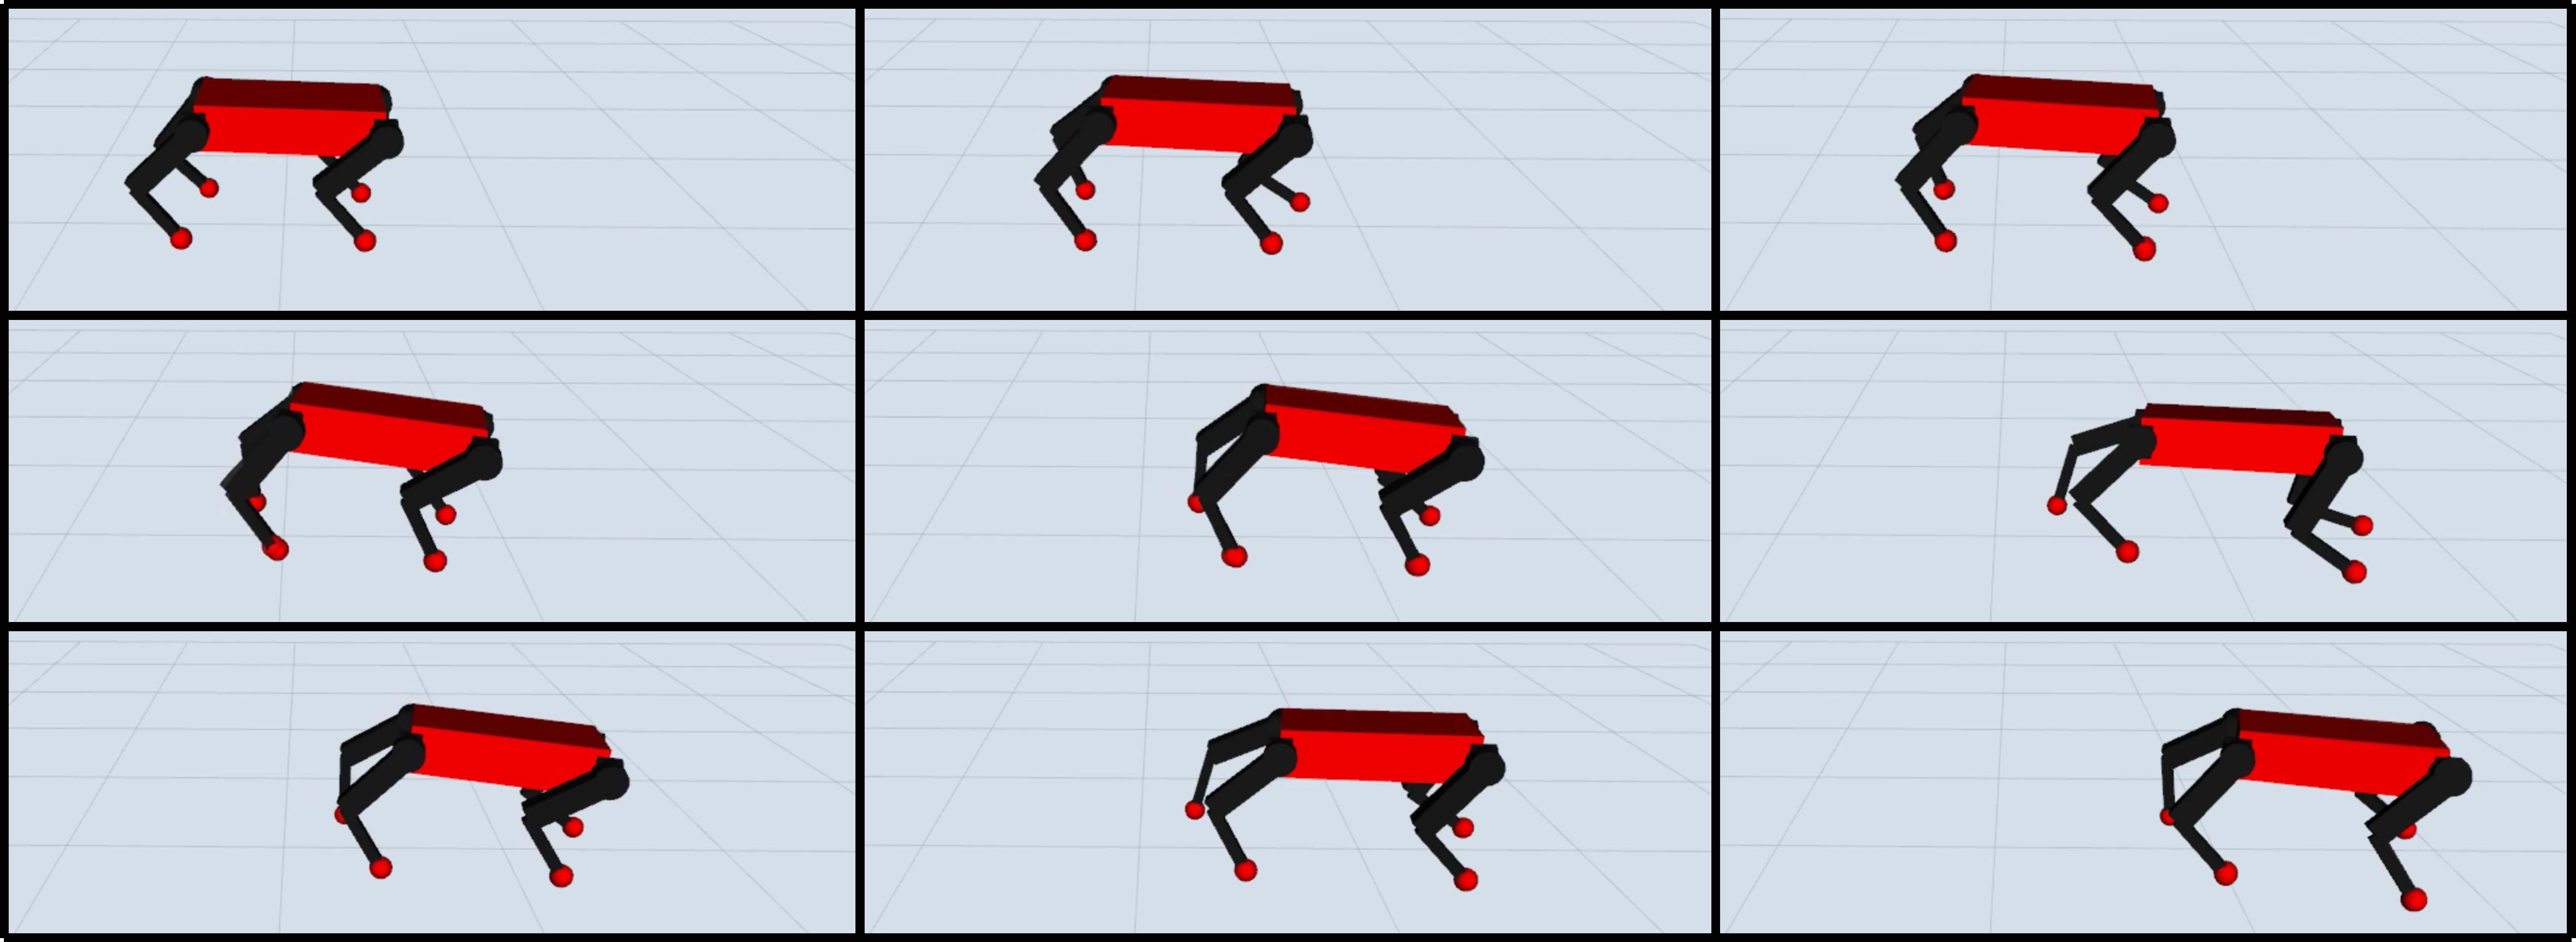
\includegraphics[width=0.8\textwidth]{docs/imgs/proof_of_concept.pdf}
\end{figure}\vskip0.3cm
\hskip0.5cm Proof of concept task:\vskip0.3cm
\begin{itemize}
	\item[$\rhd$] PPO algorithm for training
	\item[$\rhd$] Custom RHC controller for quadruped locomotion (closed source)
	\item[$\rhd$] Locomotion on flat ground exploiting RHC
	\item[$\rhd$] Act.~$\rightarrow$ agent can command the RHC through twist commands and contact phases selection
	\item[$\rhd$] Obs.~$\rightarrow$ robot orientation, meas.~twist, ref.~twist, joint positions, RHC cost and constraint violation
	\item[$\rhd$] Rew.~$\rightarrow$ 3 reward terms based on:~task error, RHC cost and constraint violation
\end{itemize}\vskip0.5cm
\end{Large}

	